\documentclass[conference]{IEEEtran}
\IEEEoverridecommandlockouts
% The preceding line is only needed to identify funding in the first footnote. If that is unneeded, please comment it out.
\usepackage{cite}
\usepackage{amsmath,amssymb,amsfonts}
\usepackage{algorithmic}
\usepackage{graphicx}
\usepackage{textcomp}
\usepackage{xcolor}
\usepackage{tabularx}
\usepackage{multirow}
\usepackage{graphics} % for pdf, bitmapped graphics files
\usepackage{subfig}
\usepackage{subcaption}
\usepackage{hyperref}
\usepackage{academicons}
\usepackage{xcolor}
\usepackage{listings}
\def\BibTeX{{\rm B\kern-.05em{\sc i\kern-.025em b}\kern-.08em
		T\kern-.1667em\lower.7ex\hbox{E}\kern-.125emX}}
	
\definecolor{codegray}{rgb}{0.5,0.5,0.5}
\definecolor{keywordblue}{rgb}{0.13,0.29,0.53}
\definecolor{stringgreen}{rgb}{0.18,0.54,0.34}

\lstset{
	language=[Sharp]C,
	basicstyle=\ttfamily\small,
	keywordstyle=\color{keywordblue}\bfseries,
	stringstyle=\color{stringgreen},
	commentstyle=\color{codegray}\itshape,
	numbers=left,
	numberstyle=\tiny\color{codegray},
	stepnumber=1,
	numbersep=10pt,
	tabsize=1,
	showspaces=false,
	showstringspaces=false,
	breaklines=true,
	breakatwhitespace=true,
	escapeinside={(*@}{@*)}
}	

% Gráficas en MATLAB
\usepackage{tikz, pgfplots}
% Color Enlace
\definecolor{colorEnlace}{RGB}{0, 0, 0}
\hypersetup{
	colorlinks=true,
	linkcolor=colorEnlace,
	citecolor=colorEnlace,
	urlcolor=colorEnlace,
	pdfauthor={Davis Bremdow Salazar Roa},
	pdftitle={}
}
% Control 
\usepackage{amsmath}
\begin{document}
	
	\title{Analizador Léxico, código de prueba}
	\author{	
		\IEEEauthorblockN{Davis Bremdow Salazar Roa}
		\IEEEauthorblockA{Universidad Nacional de San Antonio Abad del Cusco}
		\textit{Escuela Profesional de Ingeniería Electrónica}\\
		\textit{Laboratorio de Control I}\\
		200353 \\\\
		Cusco, Perú
	}
	
	\maketitle
	
	\begin{abstract}
		C\# implements a lexical analyzer to identify components like keywords, identifiers, numbers, operators, and comments within source code. It uses a finite state machine (FSM) to manage lexical states and transitions, categorizing each segment into specific tokens (using TokenType). This class enables step-by-step analysis of an input string, building a list of tokens that reflect the lexical structure of the source code.
	\end{abstract}
	
	\begin{IEEEkeywords}
		Lexical analysis, finite state machine, tokens, identifiers, operators, keywords, comments, source code, parsing, syntax
	\end{IEEEkeywords}
	
	\section{Introducción}
	La clase CScanner implementa un analizador léxico básico para identificar diferentes componentes en el código fuente, como palabras clave, identificadores, números, operadores y comentarios. Utiliza una máquina de estados finitos (FSM) para manejar distintos estados léxicos y transiciones, categorizando cada fragmento de código en tokens específicos (usando TokenType). Esta clase facilita el análisis de una cadena de entrada paso a paso, construyendo una lista de tokens que representan la estructura léxica del código fuente.
	
	\section{Analizar uno de los estados de la FSM (Finite State Machine)}
	
	En analizador de Léxico basa su funcionamiento en una maquina de estados la cual se encarga de verificar y categorizar los diferentes elementos que se pueden encontrar en un lenguaje de programación de alto nivel, para este caso en especifico la maquina de estados podrá categorizar.
	\begin{itemize}
		\item Palabras clave
		\item Identificador
		\item Numero
		\item Operador
		\item Símbolo
		\item Cadena
		\item Comentario
		\item Desconocido
		\item Fin de Archivo
	\end{itemize}
	
	Además la maquina de estado cuenta con diferentes estados que permiten realizar este proceso, siendo el caso particular para realizar su análisis, el estado \textbf{ProcesarEstadoInicio} el cual a grandes rasgos se encarga de realizar la transición al resto de estados en función al carácter de análisis actual, el código C\# para este estado se define en el listing \ref{lst:fsm-estado-inicio}
	
	\begin{lstlisting}[label=lst:fsm-estado-inicio, caption={Estado Procesar Estado Inicio de la FSM del Analizador de Lexico}, numbers=none]
		private void ProcesarEstadoInicio(char caracterActual, ref string tokenActual, List<(TokenType, string)> tokens)
		{
			// Valida si existe un espacio en blanco y un salto de linea e incrementa
			if (char.IsWhiteSpace(caracterActual))
			{
				if (caracterActual == '\n')
				{
					aLineaActual++;
				}
				// Manejo de espacios en blanco y lineas en blanco
			}
			else if (caracterActual == '#')
			{
				// Transicion al estado Comentario
				aEstadoActual = Estado.Comentario;
				tokenActual += caracterActual;
			}
			else if (char.IsLetter(caracterActual))
			{
				// char nos permite saber si se tiene una letra, para pasar al esta Identificador
				// Transicion al estado Identificador
				aEstadoActual = Estado.Identificador;
				tokenActual += caracterActual;
			}
			else if (char.IsDigit(caracterActual))
			{
				// Transicion al estado Numero
				aEstadoActual = Estado.Numero;
				tokenActual += caracterActual;
			}
			else if (Simbolos.Contains(caracterActual))
			{
				// Manejo directo de simbolos
				tokens.Add((TokenType.Sm, caracterActual.ToString()));
			}
			else if (EsInicioOperador(caracterActual))
			{
				// Transicion al estado Operador
				aEstadoActual = Estado.Operador;
				tokenActual += caracterActual;
			}
			else if (caracterActual == '"')
			{
				// Transicion al estado Cadena
				aEstadoActual = Estado.Cadena;
			}
			else
			{
				// Transicion al estado Error en caso de caracter inesperado
				aEstadoActual = Estado.Error;
				Console.WriteLine($"Error lexico en la linea {aLineaActual}: Caracter inesperado '{caracterActual}'");
			}
		}
		
	\end{lstlisting}
	
	\section{Funcionamiento general de la maquina de estados}
	
	\subsection{Inicio}
	Este es el estado inicial de la FSM. Desde aquí, se procesan todos los caracteres de entrada. Dependiendo del carácter actual, el analizador puede transitar a otros estados (comentarios, cadenas, identificadores, números, operadores o símbolos) o manejar errores. También incrementa el contador de líneas si encuentra un salto de línea.
	
	\subsection{Identificador}
	En este estado, se construyen identificadores y palabras clave. Se acepta cualquier combinación de letras, dígitos y guiones bajos. Cuando se encuentra un carácter que no forma parte de un identificador, se determina si es una palabra clave o un identificador normal y se agrega el token correspondiente a la lista de tokens.
	
	\subsection{Número}
	Este estado se encarga de reconocer números. Se permite la entrada de dígitos consecutivos. Al encontrar un carácter no numérico, se agrega el número completo como un token a la lista y se regresa al estado inicial.
	
	\subsection{Operador}
	Aquí se identifican los operadores. Si el carácter actual forma parte de un operador, se continúa construyendo el token. Cuando se completa un operador válido, se agrega a la lista de tokens. Si se encuentra un carácter que no forma parte del operador, se agrega el token si es válido, o se lanza un error si no lo es.
	
	\subsection{Símbolo}
	Este estado maneja símbolos como paréntesis, llaves y otros caracteres especiales. Cuando se encuentra un símbolo, se agrega inmediatamente a la lista de tokens sin necesidad de construir un token adicional.
	
	\subsection{Comentario}
	En este estado, el analizador ignora el contenido de un comentario de una línea. Cuando se encuentra un salto de línea, se considera que el comentario ha terminado y se agrega el token correspondiente antes de regresar al estado inicial.
	
	\subsection{Cadena}
	Este estado se utiliza para reconocer cadenas de texto. Cuando se encuentra un carácter de inicio de cadena (`"`), el analizador comienza a acumular caracteres. Si se encuentra un carácter de escape (`\`), se maneja adecuadamente. Al llegar al final de la cadena, se agrega como un token.
	
	\subsection{Error}
	Este estado se activa cuando se encuentra un carácter inesperado que no encaja en ninguna de las categorías definidas. Se informa del error y se termina el análisis.
	
	\subsection{Fin}
	Este es el estado final que indica que se ha procesado toda la entrada. No se realizan más transiciones desde este estado. Aquí se agrega un token especial que indica el fin de archivo (`EOF`).
	
	Finalmente cabe resaltar que se realizo la asignación de un función/método para cada estado de la maquina de estados del analizador léxico, siendo para el caso del estados Inicio el método ProcesarEstadoInicio, respectivamente.
	
	\section{Programa de prueba para el analizador Léxico}
	
	Para poder hacer uso de la librería previamente es necesario compilar la solución para generar la librería .dll del analizador de léxico y seguidamente crear un nuevo proyecto donde se agregará esta solución para poder hacer uso de la clase \textbf{CScanner} en donde se definió la maquina de estados con los diferentes métodos que la integran.
	
	Al tratarse \textbf{CScanner} de una clase será necesaria realizar una instancia de la clase para poder hacer uso de los métodos definidos que para el caso de esta será necesario invocar al método Analizar debido a que este se definen e invocan al resto de métodos y será el mismo que nos retorna una lista de tokens del código de entrada asignada a la clase \textbf{CScanner}.
	
	El código C\# con este código de prueba se muestra en el listing \ref{lst:codigo-prueba}
	
	\begin{lstlisting}[label=lst:codigo-prueba, caption={Codigo C\# de prueba}]
		using AnalizadorLexico;
		
		
		class Program
		{
			static void Main(string[] args)
			{
				string codigoPrograma;
				
				// codigoFuente = Console.ReadLine();
				codigoPrograma = "# Funcion saludo, retorna un string, tiene un parametro asignado\r\ndef saludar(nombre):\r\n    return \"Bienvenido\" + nombre\r\n\r\n\r\n";
				
				CScanner scanner = new CScanner(codigoPrograma);
				
				// Recuperando los tokens a partir de la funcion Analizar la cual hace uso de la FSM
				List<(CScanner.TokenType, string)> tokens = scanner.Analizar();
				
				Console.WriteLine(codigoPrograma);
				foreach ( var token in tokens)
				{
					Console.WriteLine($"{token.Item1} : {token.Item2}");
				}
				
				Console.ReadKey();
				
			}
		}
	\end{lstlisting}
	
	Como el método Analizar() retorna una lista TokenType y un string, sera necesario definir una lista de este tipo para poder recuperar la respuesta para finalmente mostrar el resultado mediante un bucle foreach el cual se encargara de recorrer cada elemento de la lista para mostrar su contendido, siendo el mismo el que se muestra en la figura \ref{fig:salida-analizar-lexico}
	
	\begin{figure}[h]
		\centering
		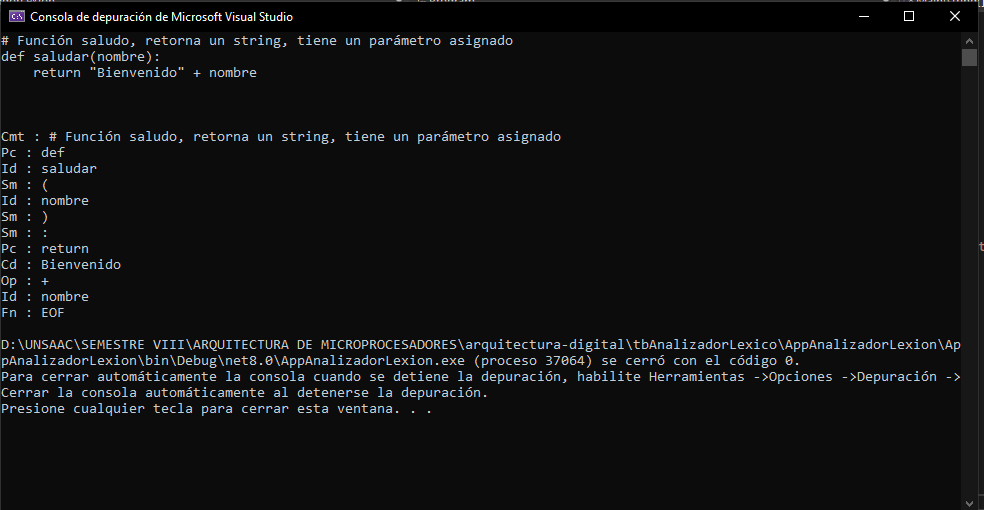
\includegraphics[width=0.5\textwidth]{media/salida-analizar-lexico}
		\caption{Salida del proyecto de prueba del Analizar Léxico}
		\label{fig:salida-analizar-lexico}
	\end{figure}
	
	
	\bibliographystyle{IEEEtran}
	\bibliography{biblio}
\end{document}
































